\documentclass[11pt,a4paper]{article}

\usepackage[utf8]{inputenc}
\usepackage[T1]{fontenc}
\usepackage[margin=2.3cm]{geometry}
\usepackage{graphicx}
\usepackage{booktabs}
\usepackage{amsmath}
\usepackage{float}
\usepackage{subcaption}
\usepackage{xcolor}
\usepackage{hyperref}
\usepackage{enumitem}

\hypersetup{
  colorlinks=true,
  linkcolor=blue!60!black,
  urlcolor=blue!60!black,
  citecolor=blue!60!black
}

\newcommand{\code}[1]{\texttt{#1}}
\newcommand{\tipt}{TIPT-v3}
\newcommand{\vitpose}{ViTPose-B}

\title{\textbf{Texture-Invariant Pose Transformer basato su ViTPose-B}\\
\large Report tecnico di implementazione, training e valutazione}
\author{Progetto TIPT}
\date{\today}

\begin{document}

\maketitle

\begin{abstract}
Questo report descrive il lavoro svolto per costruire e valutare una variante
Texture-Invariant Pose Transformer (TIPT) a partire da \vitpose. L'obiettivo
principale e' migliorare la stima della posa umana quando le immagini sono
offuscate tramite blur o pixelation, mantenendo un confronto rigoroso con la
baseline. Il lavoro ha incluso la costruzione di una pipeline COCO top-down,
l'applicazione online dell'obfuscation, una architettura shape-first con stream
strutturale dedicato, una loss di invarianza tra viste offuscate, metriche COCO
standard e un protocollo di valutazione allineato a ViTPose/Hugging Face.
\end{abstract}

\section{Obiettivo}

Il punto di partenza e' \vitpose, un modello top-down per human pose estimation
che riceve un crop persona e predice 17 heatmap COCO. La baseline e' molto forte
su immagini pulite, ma il suo flusso e' single-stream: texture, contorni e
informazioni geometriche vengono fusi negli stessi token del backbone.

L'idea TIPT e' rendere piu' esplicita la componente strutturale della persona:
non si vuole semplicemente addestrare \vitpose{} su immagini offuscate, ma
costruire una rappresentazione shape-first che resti stabile quando texture,
dettagli fini e identita' visiva vengono degradati. Per questo sono stati
introdotti:

\begin{itemize}[leftmargin=1.2em]
  \item obfuscation online, senza salvare dataset duplicati;
  \item uno stream strutturale basato su edge map;
  \item una fusione residua shape-texture ripetuta su piu' blocchi;
  \item una loss di invarianza fra due viste offuscate della stessa istanza;
  \item uno sweep sistematico su intensita' di blur e pixelation.
\end{itemize}

\section{Pipeline dati}

La pipeline usa COCO keypoints in modalita' top-down con bounding box persona
prese dalle annotation COCO. Ogni elemento del dataset produce:

\begin{itemize}[leftmargin=1.2em]
  \item crop persona di dimensione $256 \times 192$;
  \item target heatmap $64 \times 48$ per i 17 keypoint COCO;
  \item visibility mask per la loss pesata;
  \item metadati COCO per riportare le predizioni in coordinate immagine.
\end{itemize}

L'obfuscation e' applicata durante il data loading. Questo evita di materializzare
piu' copie del dataset e permette di cambiare intensita' o tipo di degradazione
in training/evaluation. Sono supportate tre modalita':

\begin{itemize}[leftmargin=1.2em]
  \item \code{none}: crop pulito;
  \item \code{blur}: Gaussian blur parametrizzato tramite kernel size dispari;
  \item \code{pixelate}: downsample/upsample nearest-neighbor parametrizzato da pixel size.
\end{itemize}

Per il blur, il parametro usato nel config e' \code{blur\_kernel\_size}. Se si
usa un range, ad esempio $[3,17]$, vengono campionati solo valori dispari:
$3,5,7,\dots,17$. Internamente il kernel size viene convertito nel raggio usato
da PIL con:

\[
  r = \frac{k - 1}{6}.
\]

Per la pixelation, \code{pixel\_size} indica la dimensione del blocco in pixel:
un valore alto distrugge piu' dettaglio locale.

\section{Architettura}

La baseline \vitpose{} usa un singolo flusso:

\[
  I_{\mathrm{rgb}} \rightarrow \mathrm{PatchEmbed}
  \rightarrow \mathrm{ViTBackbone}
  \rightarrow \mathrm{HeatmapDecoder}.
\]

In \tipt{}, invece, l'input viene elaborato in due stream:

\begin{itemize}[leftmargin=1.2em]
  \item \textbf{texture/context stream}: il backbone pretrained di \vitpose{}
  produce token $F_{\mathrm{tex}}$;
  \item \textbf{structural stream}: dal crop normalizzato vengono estratti
  canali strutturali \code{sobel\_x}, \code{sobel\_y} e \code{magnitude}; questi
  passano in una piccola CNN 3x3 e in una patch embedding che produce
  $F_{\mathrm{shape}}$.
\end{itemize}

La fusione e' shape-first: il percorso residuo principale resta
$F_{\mathrm{shape}}$, mentre la texture viene usata come contesto ausiliario
tramite cross-attention. Ogni blocco applica:

\[
  F_{\mathrm{shape}} \leftarrow
  F_{\mathrm{shape}} +
  g(F_{\mathrm{shape}})\,
  \mathrm{CrossAttn}
  \left(
    Q=F_{\mathrm{shape}},
    K=F_{\mathrm{tex}},
    V=F_{\mathrm{tex}}
  \right),
\]

dove $g(\cdot)$ e' un gate dinamico image-conditioned. Questa scelta evita di
ritornare a un semplice ViTPose texture-first: la texture corregge la shape, ma
non sostituisce il percorso strutturale.

\begin{figure}[H]
  \centering
  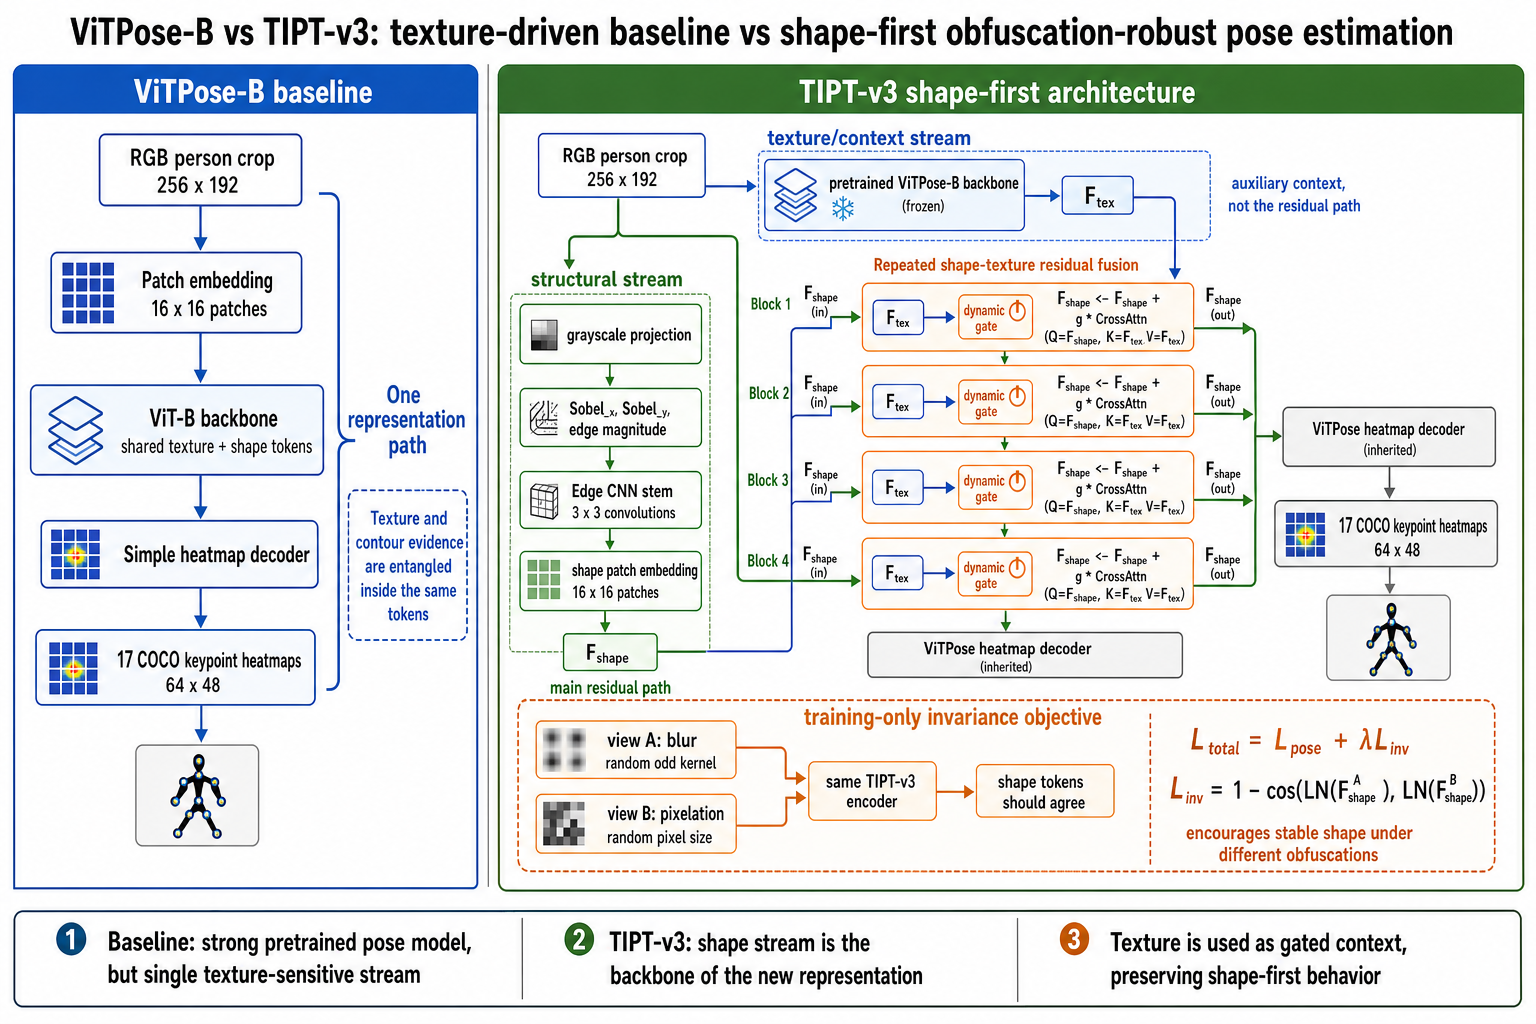
\includegraphics[width=\textwidth]{figures/architecture/tipt_vs_vitpose_architecture.png}
  \caption{Confronto architetturale fra \vitpose{} e \tipt{}. La baseline e'
  single-stream; \tipt{} introduce uno stream strutturale shape-first e una
  fusione residua guidata da cross-attention.}
  \label{fig:architecture}
\end{figure}

\section{Loss e training}

La loss principale e' la mean squared error pesata sulle heatmap:

\[
  \mathcal{L}_{\mathrm{pose}} =
  \frac{1}{N}
  \sum_{i,k,u,v}
  w_{i,k}
  \left(
    \hat{H}_{i,k,u,v} - H_{i,k,u,v}
  \right)^2,
\]

dove $w_{i,k}$ e' la visibility mask del keypoint $k$.

La parte specifica di \tipt{} e' la training objective two-view. Per ogni crop
vengono create due viste offuscate della stessa istanza:

\[
  I^A = \mathrm{blur}(I), \qquad
  I^B = \mathrm{pixelate}(I).
\]

Il modello predice le heatmap su entrambe le viste e produce due rappresentazioni
shape:

\[
  F_{\mathrm{shape}}^A, \quad F_{\mathrm{shape}}^B.
\]

La loss di invarianza usata in \tipt{} e':

\[
  \mathcal{L}_{\mathrm{inv}} =
  1 -
  \cos\left(
    \mathrm{LN}(F_{\mathrm{shape}}^A),
    \mathrm{LN}(F_{\mathrm{shape}}^B)
  \right).
\]

La loss totale diventa:

\[
  \mathcal{L}_{\mathrm{total}} =
  \mathcal{L}_{\mathrm{pose}} +
  \lambda \mathcal{L}_{\mathrm{inv}},
\]

con valore di default:

\[
  \lambda = 0.05.
\]

Il senso di $\lambda$ e' controllare quanto il training debba forzare lo stream
shape a restare stabile fra blur e pixelation. Se $\lambda=0$, \tipt{} si riduce
a un training pose-only. Se $\lambda$ e' troppo alto, il modello puo' perdere
dettagli utili per localizzare i keypoint. Il valore $0.05$ e' stato scelto come
compromesso iniziale.

\section{Implementazione}

I file principali sono:

\begin{itemize}[leftmargin=1.2em]
  \item \code{models/tipt\_vitpose\_v3.py}: architettura shape-first, stream
  strutturale, CNN stem, blocchi residui shape-texture e decoder ViTPose;
  \item \code{data/coco\_keypoints.py}: dataset COCO top-down con crop persona,
  obfuscation online e viste multiple per invariance training;
  \item \code{data/transforms.py}: crop affine ViTPose, trasformazioni keypoint,
  blur e pixelation;
  \item \code{train.py}: training loop, freeze iniziale del pretrained, loss di
  invarianza, summary JSON e timing;
  \item \code{eval\_coco.py}: evaluation COCO con metriche standard AP/AR;
  \item \code{scripts/eval\_obfuscation\_sweep.py}: sweep pulita su clean, blur
  e pixelation;
  \item \code{scripts/visualize\_obfuscated\_comparison.py}: generazione di
  pannelli qualitativi baseline vs \tipt{}.
\end{itemize}

\subsection{Protocollo di valutazione}

Un problema importante emerso durante il lavoro e' stato il gap fra la baseline
misurata internamente e il valore ufficiale di \vitpose. Inizialmente la
valutazione usava:

\begin{itemize}[leftmargin=1.2em]
  \item crop/resize PIL semplice;
  \item decoding argmax grezzo sulle heatmap.
\end{itemize}

Questo produceva una AP clean della baseline intorno a $0.703$, troppo bassa
rispetto al valore atteso. Il protocollo e' stato quindi corretto introducendo:

\begin{itemize}[leftmargin=1.2em]
  \item \code{crop\_method: vitpose}: crop affine top-down compatibile con
  ViTPose;
  \item \code{decode: hf}: post-processing Hugging Face/ViTPose con DARK
  unbiased decoding;
  \item \code{dark\_kernel\_size: 11}.
\end{itemize}

Con questo protocollo, la baseline clean raggiunge $0.7634$ AP, coerente con il
risultato ufficiale. Da questo punto in poi, tutti i confronti devono usare lo
stesso evaluator anche su dati offuscati.

\section{Risultati}

\subsection{Training \tipt{}}

La run principale \tipt{} e' stata addestrata per 5 epoch con:

\begin{itemize}[leftmargin=1.2em]
  \item checkpoint iniziale \code{usyd-community/vitpose-base-simple};
  \item batch size 16;
  \item 2 epoch iniziali con pesi pretrained congelati;
  \item learning rate nuovi moduli $10^{-4}$;
  \item learning rate pretrained $10^{-5}$;
  \item invariance weight $\lambda=0.05$.
\end{itemize}

Con il vecchio evaluator, la final COCO eval su blur kernel 11 era:

\begin{center}
\begin{tabular}{lccc}
\toprule
Modello & AP & AP50 & AP75 \\
\midrule
\tipt{} su blur $k=11$ & 0.7002 & 0.9221 & 0.7949 \\
\bottomrule
\end{tabular}
\end{center}

Questi numeri restano utili storicamente, ma non devono essere confrontati con
la baseline ufficiale-like dopo la correzione del protocollo.

\subsection{Valutazione clean con protocollo ViTPose/HF}

\begin{center}
\begin{tabular}{lcccc}
\toprule
Modello & AP & AP50 & AP75 & PCK \\
\midrule
\vitpose{} baseline & 0.7634 & 0.9321 & 0.8399 & 0.9148 \\
\tipt{} checkpoint esistente & 0.7166 & 0.9325 & 0.8058 & 0.9139 \\
\bottomrule
\end{tabular}
\end{center}

Questo risultato e' coerente: su immagini pulite la baseline pretrained rimane
piu' forte. Il checkpoint \tipt{} esistente e' pero' stato addestrato prima della
correzione del crop affine, quindi questo confronto contiene un piccolo mismatch
train/eval. Per una misura definitiva occorre riaddestrare \tipt{} con
\code{crop\_method: vitpose}.

\subsection{Sweep preliminare su blur}

Prima della correzione del protocollo ufficiale-like, era stata eseguita una
sweep su blur con kernel dispari da 3 a 17. Anche se i valori assoluti vanno
ricalcolati con il nuovo evaluator, il trend era molto chiaro:

\begin{center}
\begin{tabular}{rrrr}
\toprule
Kernel blur & AP \vitpose{} & AP \tipt{} & Guadagno \tipt{} \\
\midrule
3  & 0.7033 & 0.7229 & +0.0196 \\
5  & 0.6993 & 0.7198 & +0.0205 \\
7  & 0.6886 & 0.7130 & +0.0244 \\
9  & 0.6709 & 0.7071 & +0.0361 \\
11 & 0.6537 & 0.7002 & +0.0465 \\
13 & 0.6316 & 0.6919 & +0.0603 \\
15 & 0.6080 & 0.6786 & +0.0706 \\
17 & 0.5857 & 0.6665 & +0.0807 \\
\bottomrule
\end{tabular}
\end{center}

Il comportamento interessante e' che il vantaggio di \tipt{} cresce con
l'intensita' del blur. Questo e' esattamente il segnale atteso da una
architettura shape-first: quando la texture viene degradata, la baseline perde
piu' rapidamente.

\section{Esempi qualitativi}

Le figure seguenti mostrano confronti qualitativi generati su crop COCO
offuscati. In ogni pannello: input offuscato, predizione \vitpose, predizione
\tipt{} e ground truth. Le linee rosse indicano la predizione; le linee verdi
indicano il target COCO.

\begin{figure}[H]
  \centering
  \begin{subfigure}{0.98\textwidth}
    \centering
    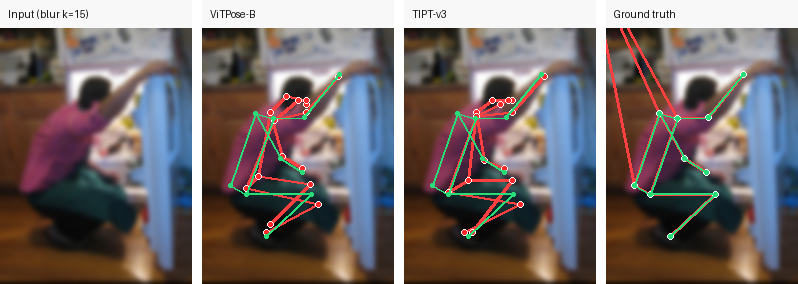
\includegraphics[width=\textwidth]{figures/inference_examples/blur_sample_000000_image_425226_ann_183126.png}
    \caption{Blur, kernel 15, sample 0.}
  \end{subfigure}
  \vspace{0.3cm}
  \begin{subfigure}{0.98\textwidth}
    \centering
    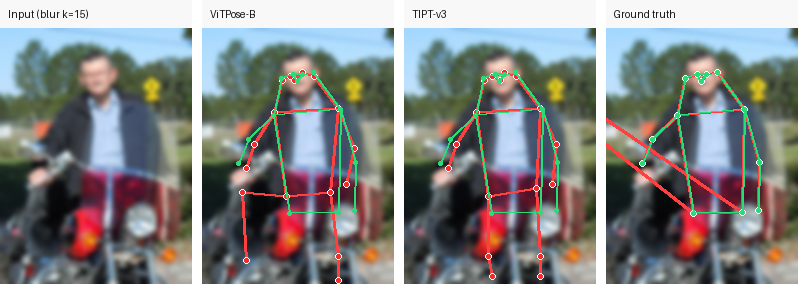
\includegraphics[width=\textwidth]{figures/inference_examples/blur_sample_000010_image_481567_ann_186174.png}
    \caption{Blur, kernel 15, sample 10.}
  \end{subfigure}
  \caption{Confronto qualitativo su immagini blur.}
  \label{fig:blur_examples}
\end{figure}

\begin{figure}[H]
  \centering
  \begin{subfigure}{0.98\textwidth}
    \centering
    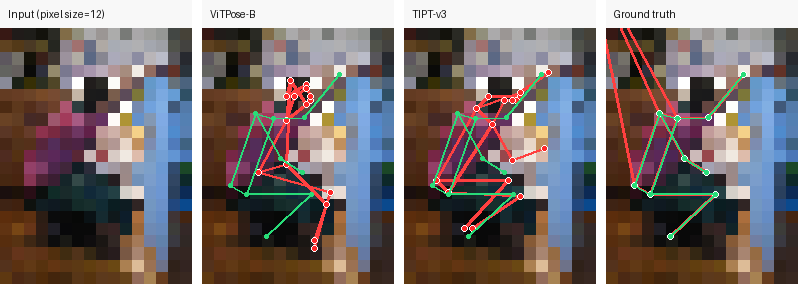
\includegraphics[width=\textwidth]{figures/inference_examples/pixelate_sample_000000_image_425226_ann_183126.png}
    \caption{Pixelation, pixel size 12, sample 0.}
  \end{subfigure}
  \vspace{0.3cm}
  \begin{subfigure}{0.98\textwidth}
    \centering
    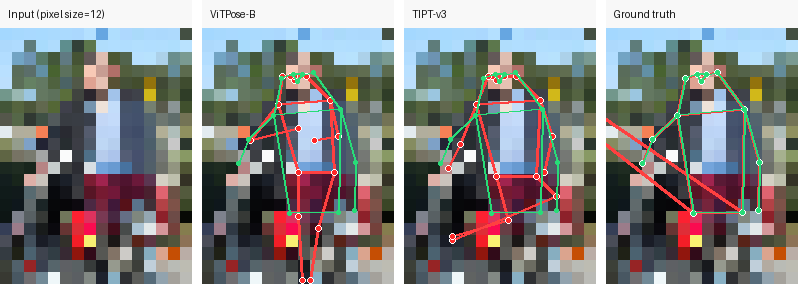
\includegraphics[width=\textwidth]{figures/inference_examples/pixelate_sample_000010_image_481567_ann_186174.png}
    \caption{Pixelation, pixel size 12, sample 10.}
  \end{subfigure}
  \caption{Confronto qualitativo su immagini pixelate.}
  \label{fig:pixel_examples}
\end{figure}

\section{Perche' queste scelte}

\paragraph{Obfuscation online.}
Permette di cambiare intensita' e tipo di degradazione senza creare dataset
duplicati. Questo rende pratici gli sweep e riduce spazio occupato su disco.

\paragraph{Stream strutturale.}
L'edge magnitude e i gradienti Sobel enfatizzano contorni e silhouette, cioe'
informazioni piu' stabili rispetto alla texture fine quando si applicano blur o
pixelation.

\paragraph{CNN prima delle patch.}
La CNN 3x3 sullo stream edge serve a costruire feature locali prima della
patchification. Senza questo passaggio, i token strutturali nascerebbero da edge
map troppo grezze e locali.

\paragraph{Shape-first residual fusion.}
La formula residua mantiene $F_{\mathrm{shape}}$ come stato principale. Questo
e' importante per evitare che il modello degeneri in una variante quasi uguale a
\vitpose{} base.

\paragraph{Invariance loss.}
La loss two-view forza la rappresentazione shape a restare simile quando la
stessa posa viene vista con due degradazioni diverse. In questo modo il modello
non impara solo a riconoscere uno specifico blur, ma viene spinto a costruire
una rappresentazione piu' stabile.

\section{Limiti attuali e prossimi passi}

\begin{itemize}[leftmargin=1.2em]
  \item Il checkpoint \tipt{} principale e' stato addestrato prima della
  correzione \code{crop\_method: vitpose}; va riaddestrato con il nuovo
  protocollo.
  \item Gli sweep blur/pixelation devono essere rieseguiti con
  \code{decode: hf} e \code{crop\_method: vitpose}.
  \item Il risultato clean non e' l'obiettivo principale: e' normale che
  \vitpose{} resti superiore su immagini non offuscate. La domanda chiave e':
  quanto perde ogni modello quando cresce l'intensita' dell'obfuscation?
  \item Sarebbe utile loggare statistiche dei gate dinamici per capire quanto
  ogni blocco usa texture context.
  \item Una futura versione potrebbe estrarre $F_{\mathrm{tex}}$ da piu' livelli
  intermedi del backbone ViTPose, non solo dall'ultimo feature map.
\end{itemize}

\section{Comandi principali}

Training \tipt{}:

\begin{verbatim}
.venv/bin/python train.py --config configs/tipt_vitpose_v3_hf_coco.yaml
\end{verbatim}

Valutazione clean baseline:

\begin{verbatim}
.venv/bin/python eval_coco.py \
  --config configs/vitpose_b_baseline_hf_coco.yaml \
  --obfuscation none \
  --metrics-json runs/baseline_vitpose_b_clean_hf_metrics.json \
  --results-json runs/baseline_vitpose_b_clean_hf_preds.json
\end{verbatim}

Sweep completo clean/blur/pixelation:

\begin{verbatim}
.venv/bin/python scripts/eval_obfuscation_sweep.py \
  --baseline-config configs/vitpose_b_baseline_hf_coco.yaml \
  --tipt-config configs/tipt_vitpose_v3_hf_coco.yaml \
  --sweeps clean blur pixelate \
  --blur-min-kernel 3 \
  --blur-max-kernel 17 \
  --pixel-sizes 4 6 8 10 12 16 \
  --plot
\end{verbatim}

Esempi qualitativi:

\begin{verbatim}
.venv/bin/python scripts/visualize_obfuscated_comparison.py \
  --tipt-checkpoint runs/tipt_vitpose_v3/.../best.pt \
  --obfuscation blur \
  --blur-kernel-size 15 \
  --indices 0 10
\end{verbatim}

\section{Conclusione}

Il lavoro ha trasformato un primo wrapper TIPT in una pipeline sperimentale piu'
solida: architettura shape-first, obfuscation online, loss di invarianza,
metriche COCO standard, sweep automatiche e protocollo di valutazione allineato
a ViTPose. Il risultato piu' importante non e' battere \vitpose{} sulle immagini
clean, ma mostrare una minore degradazione al crescere dell'obfuscation. Le
sweep preliminari indicano proprio questa direzione; il prossimo passo e'
riaddestrare e rivalutare tutto con il nuovo evaluator ufficiale-like.

\end{document}
